\chapter{Evaluation}
\label{cha:eval}
In this chapter, the intersection of the patent database from the Flemming's research and the engineering and scientist patent dataset from the work done by by Chunmian et al is used to evaluate the performance of my approach.  In section 5.1, the detail of the dataset would be introduced. In section 5.2, the measurements of the performance of my approach are described. In the section 5.3, the evaluation result and the explanation of the result are given. 

\section{Dataset}
The dataset used for evaluation is the intersection part of the patent database from the Flemming's work and the the engineer and scientist (E\&S) dataset from the the work done by Chunmian et al. The Flemming's database contains the inventor-patent instances from USPTO of the period from 1975 to 2010. This inventor-patent instances have been preprocessed by Flemming's approach. The Flemming's database provides a lot of useful information for the inventor-patent instances such as the patent assignee number, longitude and latitude which cannot be extracted from the patent document. The E\&S dataset contains the inventor identification information for each inventor of inventor-patent instance.  The intersection set of the two dataset contains 32495 patent-inventor units. The patent texts are extracted by using the patent full-text search engine developed by the USPTO.  The publication information is extracted from the Europe PMC by using its search engine. Another benchmark dataset used by Flemming for evaluation is also used to compare my approach with the Flemming's. Because the publication database used for evaluation is the Europe PMC which only contains the bio-medical publications, the subset of the intersection dataset which extracts the patent-inventor units from the biomedical field by using the technology class of the USPTO is used to evaluate the patent-publication matching performance. This subset contains 3605 patent-inventor units. 

\section{Measurement}
There are five measurements to evaluate the accuracy of my approach for the inventor identification. They are "F-measurement" or "F-Score", "lumping error" , "splitting Errror", "precision" and "recall" .  In order to calculate these measurements, four basic values should be calculated first based on the clustering result. They are true positive, false positive, true negative and false negative.  After clustering, each cluster contains some instances which are hoped to have the same inventor ID. The dataset for evaluation would assign each instance an inventor ID as the true value.  Within one cluster, the pairs of the instances with the same ID are considered to be correct and the other pairs are considered to be incorrect. For different clusters, the pairs of the instances are considered to be correct and the others are considered to be incorrect. The table 5.1 shows the methods to calculate the four basic values based on the number of the correct pairs and the incorrect pairs.
\begin{table}
\centering
\begin{tabular}{|c|c|c|}
\hline
 & Same Cluster & Different Clusers \\
 \hline
 Same ID & True Positive(TP) & False Negative(FN)  \\
 \hline
Different IDs & False Positive(FP) & True Negative(TN) \\
\hline
\end{tabular}
\caption{Four Basic Values For Evaluation}
\end{table}
After calculating the four basic values, the \emph{precision} and the \emph{recall} are calculated and the F-measurement is calculated based on the \emph{precision} and \emph{recall}. 
\begin{equation}
Precision =\frac{TP}{TP+FP}
\end{equation} 
\begin{equation}
Recall =\frac{TP}{TP+FN}
\end{equation} 
\begin{equation}
F-Meansurent= \frac{2}{\frac{1}{Precision}+\frac{1}{Recall}}
\end{equation}
\emph{Precision} represents fraction of the patent-inventor instances which have the same inventor ID in all the clusters and \emph{recall} represents the fraction of the inventor-patent instances which have the same ID have been put in the same cluster.The \emph{F-Measurement} is the harmonic mean of the \emph{precision} and \emph{recall} which consider both the precision and recall and is the main measurement to evaluate the performance.  The four basic value can also be used to computer another two values: \emph{lumping error} and \emph{splitting error}.
\begin{equation}
Lumping=\frac{FP}{TP+FN}
\end{equation}
\begin{equation}
Splitting=\frac{FN}{TP+FN}
\end{equation}
\emph{Lumping Error} occurs when the instances from different inventors are grouped in the same cluster while the \emph{Splitting Error} occurs when the instances from the same person are grouped into different clusters. Flemming points out the lumping error and splitting error are more intuitive and they are negative correlated. From the definition, a good result for the inventor identification should have the small values for the \emph{lumping error} and \emph{splitting error} and high values for the \emph{F-measurement}, \emph{precision} and \emph{recall}.

\section{Evaluation}
The machine used for the evaluation is Mac-mini with Mac-OS operation system. The CPU is Intel Core i5 (3M Cache, up to 2.6GHz). The RAM is 8GB. The evaluation for my thesis approach is divided into 5 parts. The intersection of inventor-patent instance dataset is divided into two datasets, training dataset and the testing dataset. The training dataset randomly picked 8000 instances from the intersection of the inventor-patent instance databases. The rest of the intersection is used as the testing dataset. The first part uses this 8000 instances to do the training and cross-validation for the evaluation of the logistic regression. The second part would randomly pick 5000 instances from the testing dataset to test the transitivity effect on the clustering result. The third part is to test the clustering performance on the testing dataset by using the values of the parameters from the first part of the evaluation.   The fourth part  compares my approach with the Flemming's approach by using the benchmark dataset. The last part of evaluation tests the patent-publication matching effect on the clustering result.

\subsection{Cross Validation for Logistic Regression}
In the first part of the evaluation, the training instance dataset which contains 8000 instances is used for cross validation. For each time, subsets with different sizes are randomly extracted from the training dataset. A 5-folder cross validation is performed on the extracted subset of the dataset. For each iteration of the cross validation, a logistic regression is performed first to get the weights and threshold. The weights and the threshold are used by hierarchical clustering and DBSCAN. The five measurements are calculated for the clustering result. For different sizes of the subsets, the standard errors and the mean values of the five measurements are also calculated to test the stabilities of the logistic regression with the clustering. The size of the subset of the training data changes from 2000 to 8000 and the increment is 2000. The hierarchical clustering uses the single linkage clustering method and the minPts of the DBSCAN is one in the first part of evaluation. Figure 5.1 and Figure 5.2 shows the mean values of measurements plot with respect to the subset size for hierarchical clustering and DBSCAN separately. From the plot, the points in the plot represent the mean values for the measurements and the lines represent the two times of the standard error of the measurements. From the result of the cross validation, the single linkage clustering have the exact the same result as the DBSCAN with minPts of 1. The reason is that both of them result in a chain rule\footnote{Chain Rule: If A is similar to B and B is similar to C, A is similar to C.} for the inventor identity. The F-measurement, precision and recall are all more than 0.99 and the standard error is less than 0.01. The lumping error and splitting error are both less than 0.01 and the standard error is also less than 0.01. 

\begin{figure}
\centering
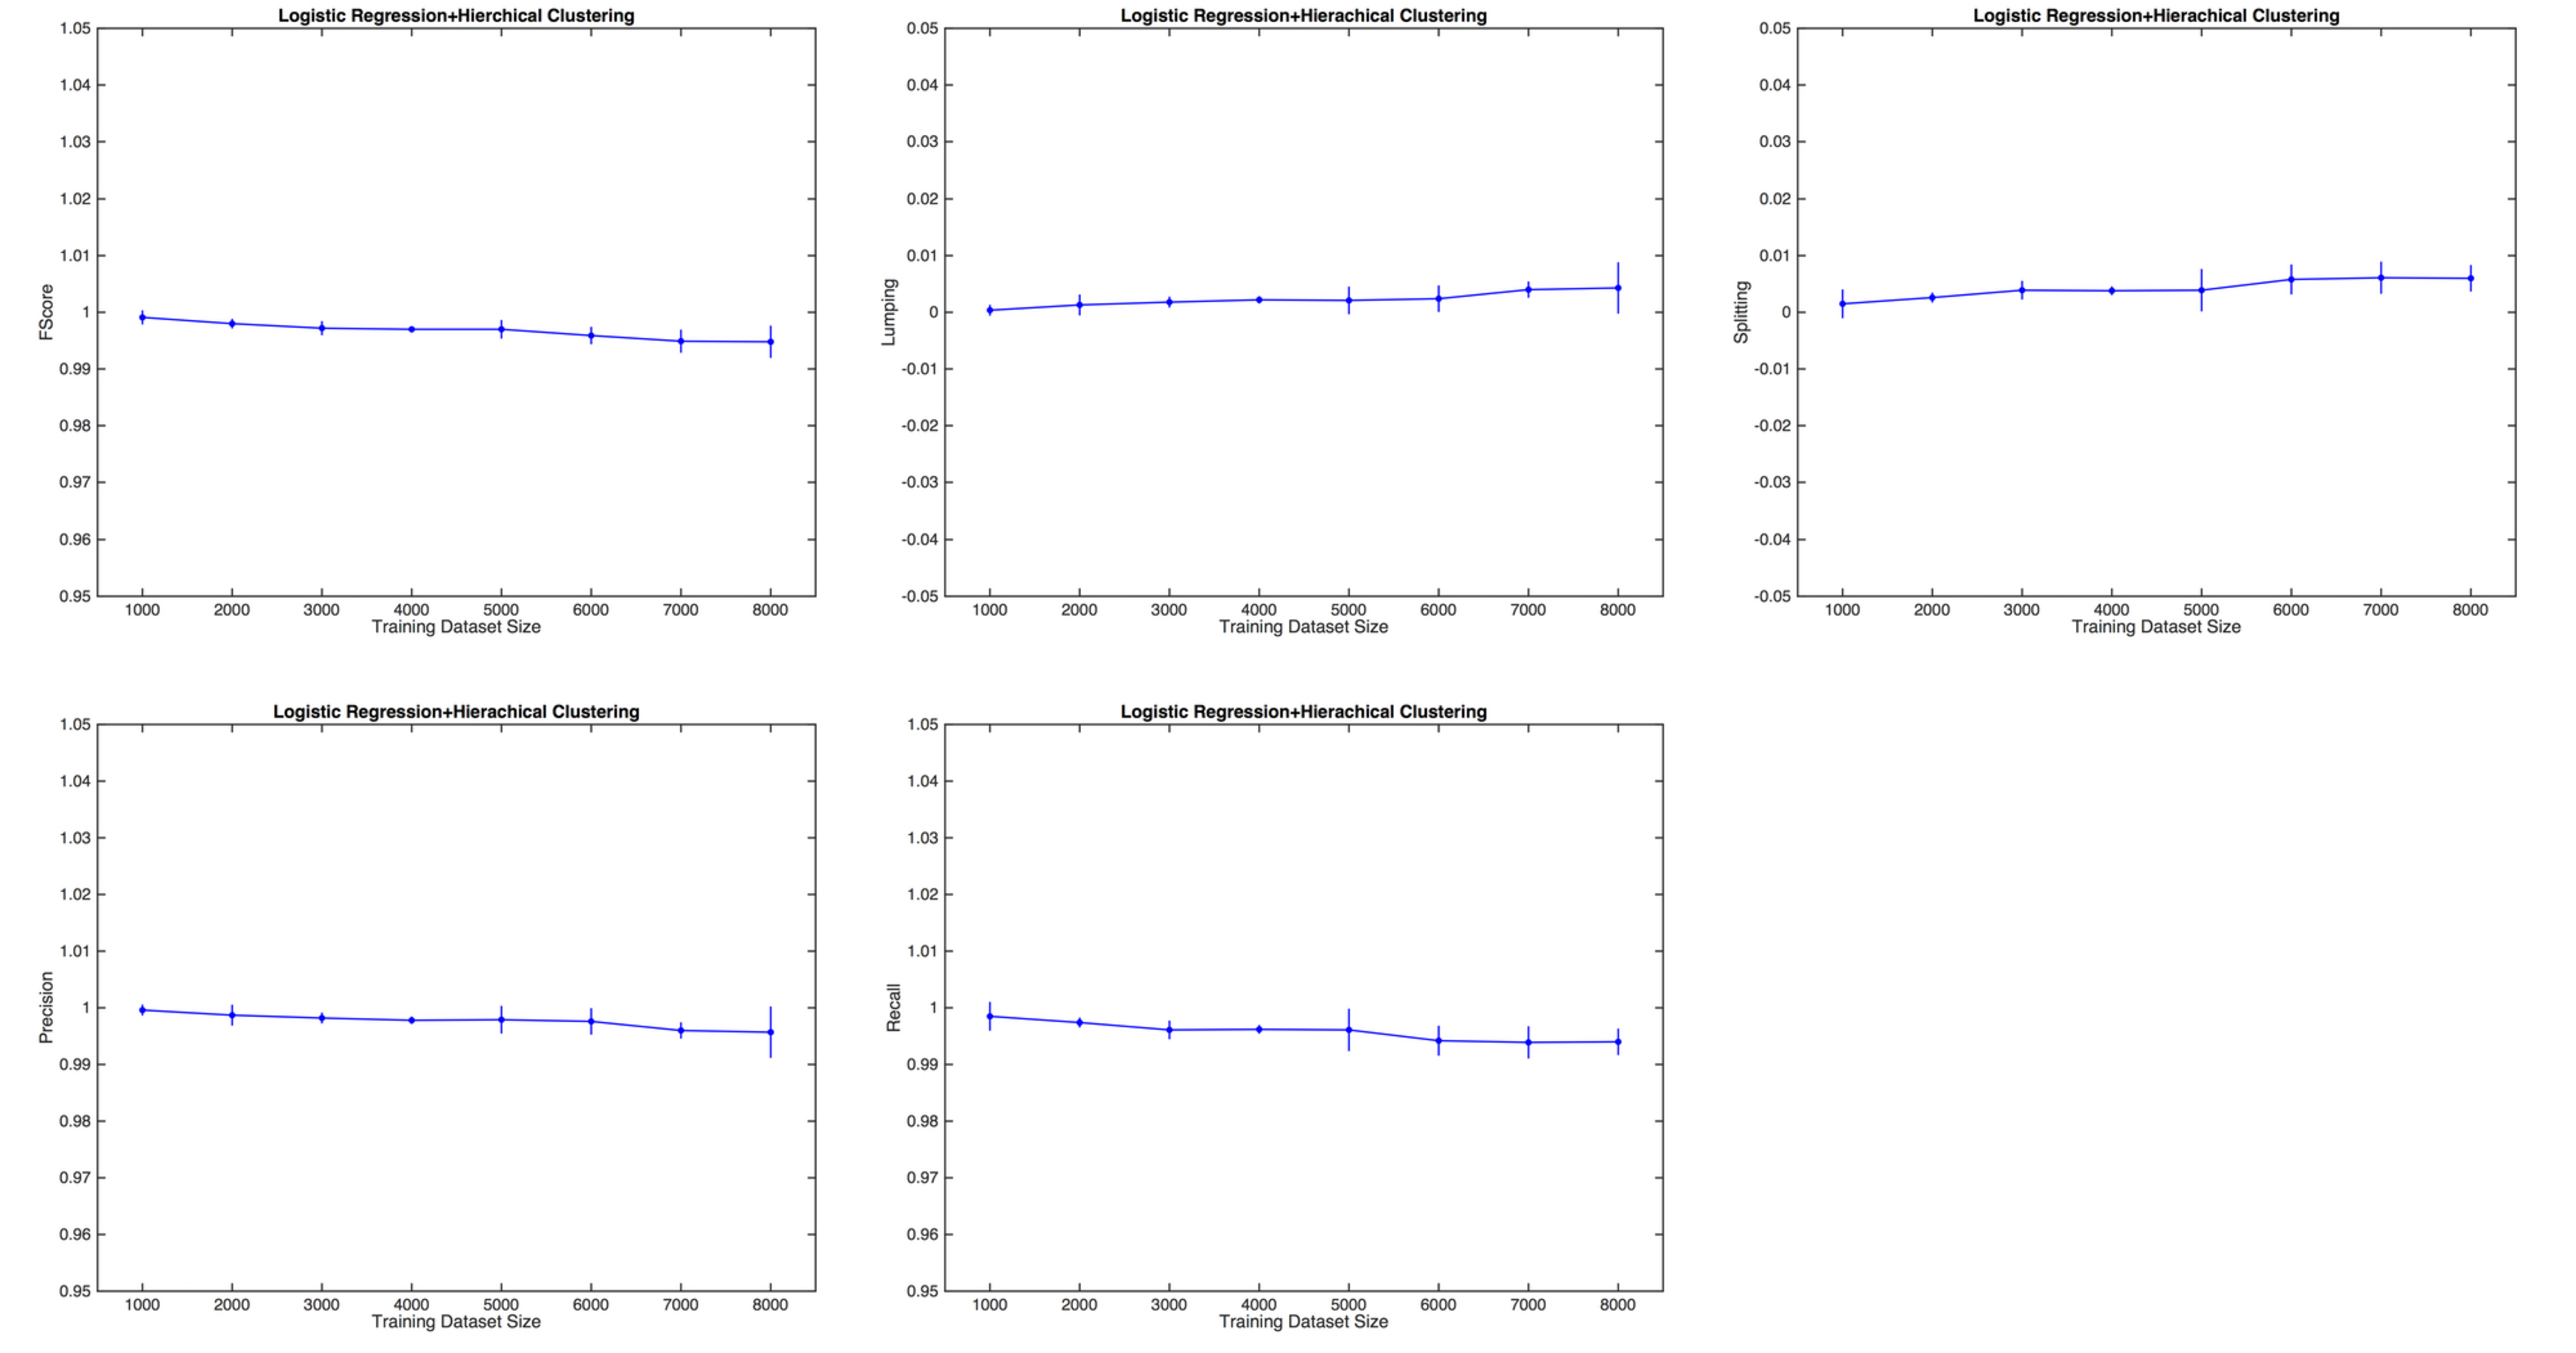
\includegraphics[scale=0.23]{CVHi.pdf}
\caption{Cross Validation for the Hierarchical Clustering}
\end{figure}
\begin{figure} 
\centering
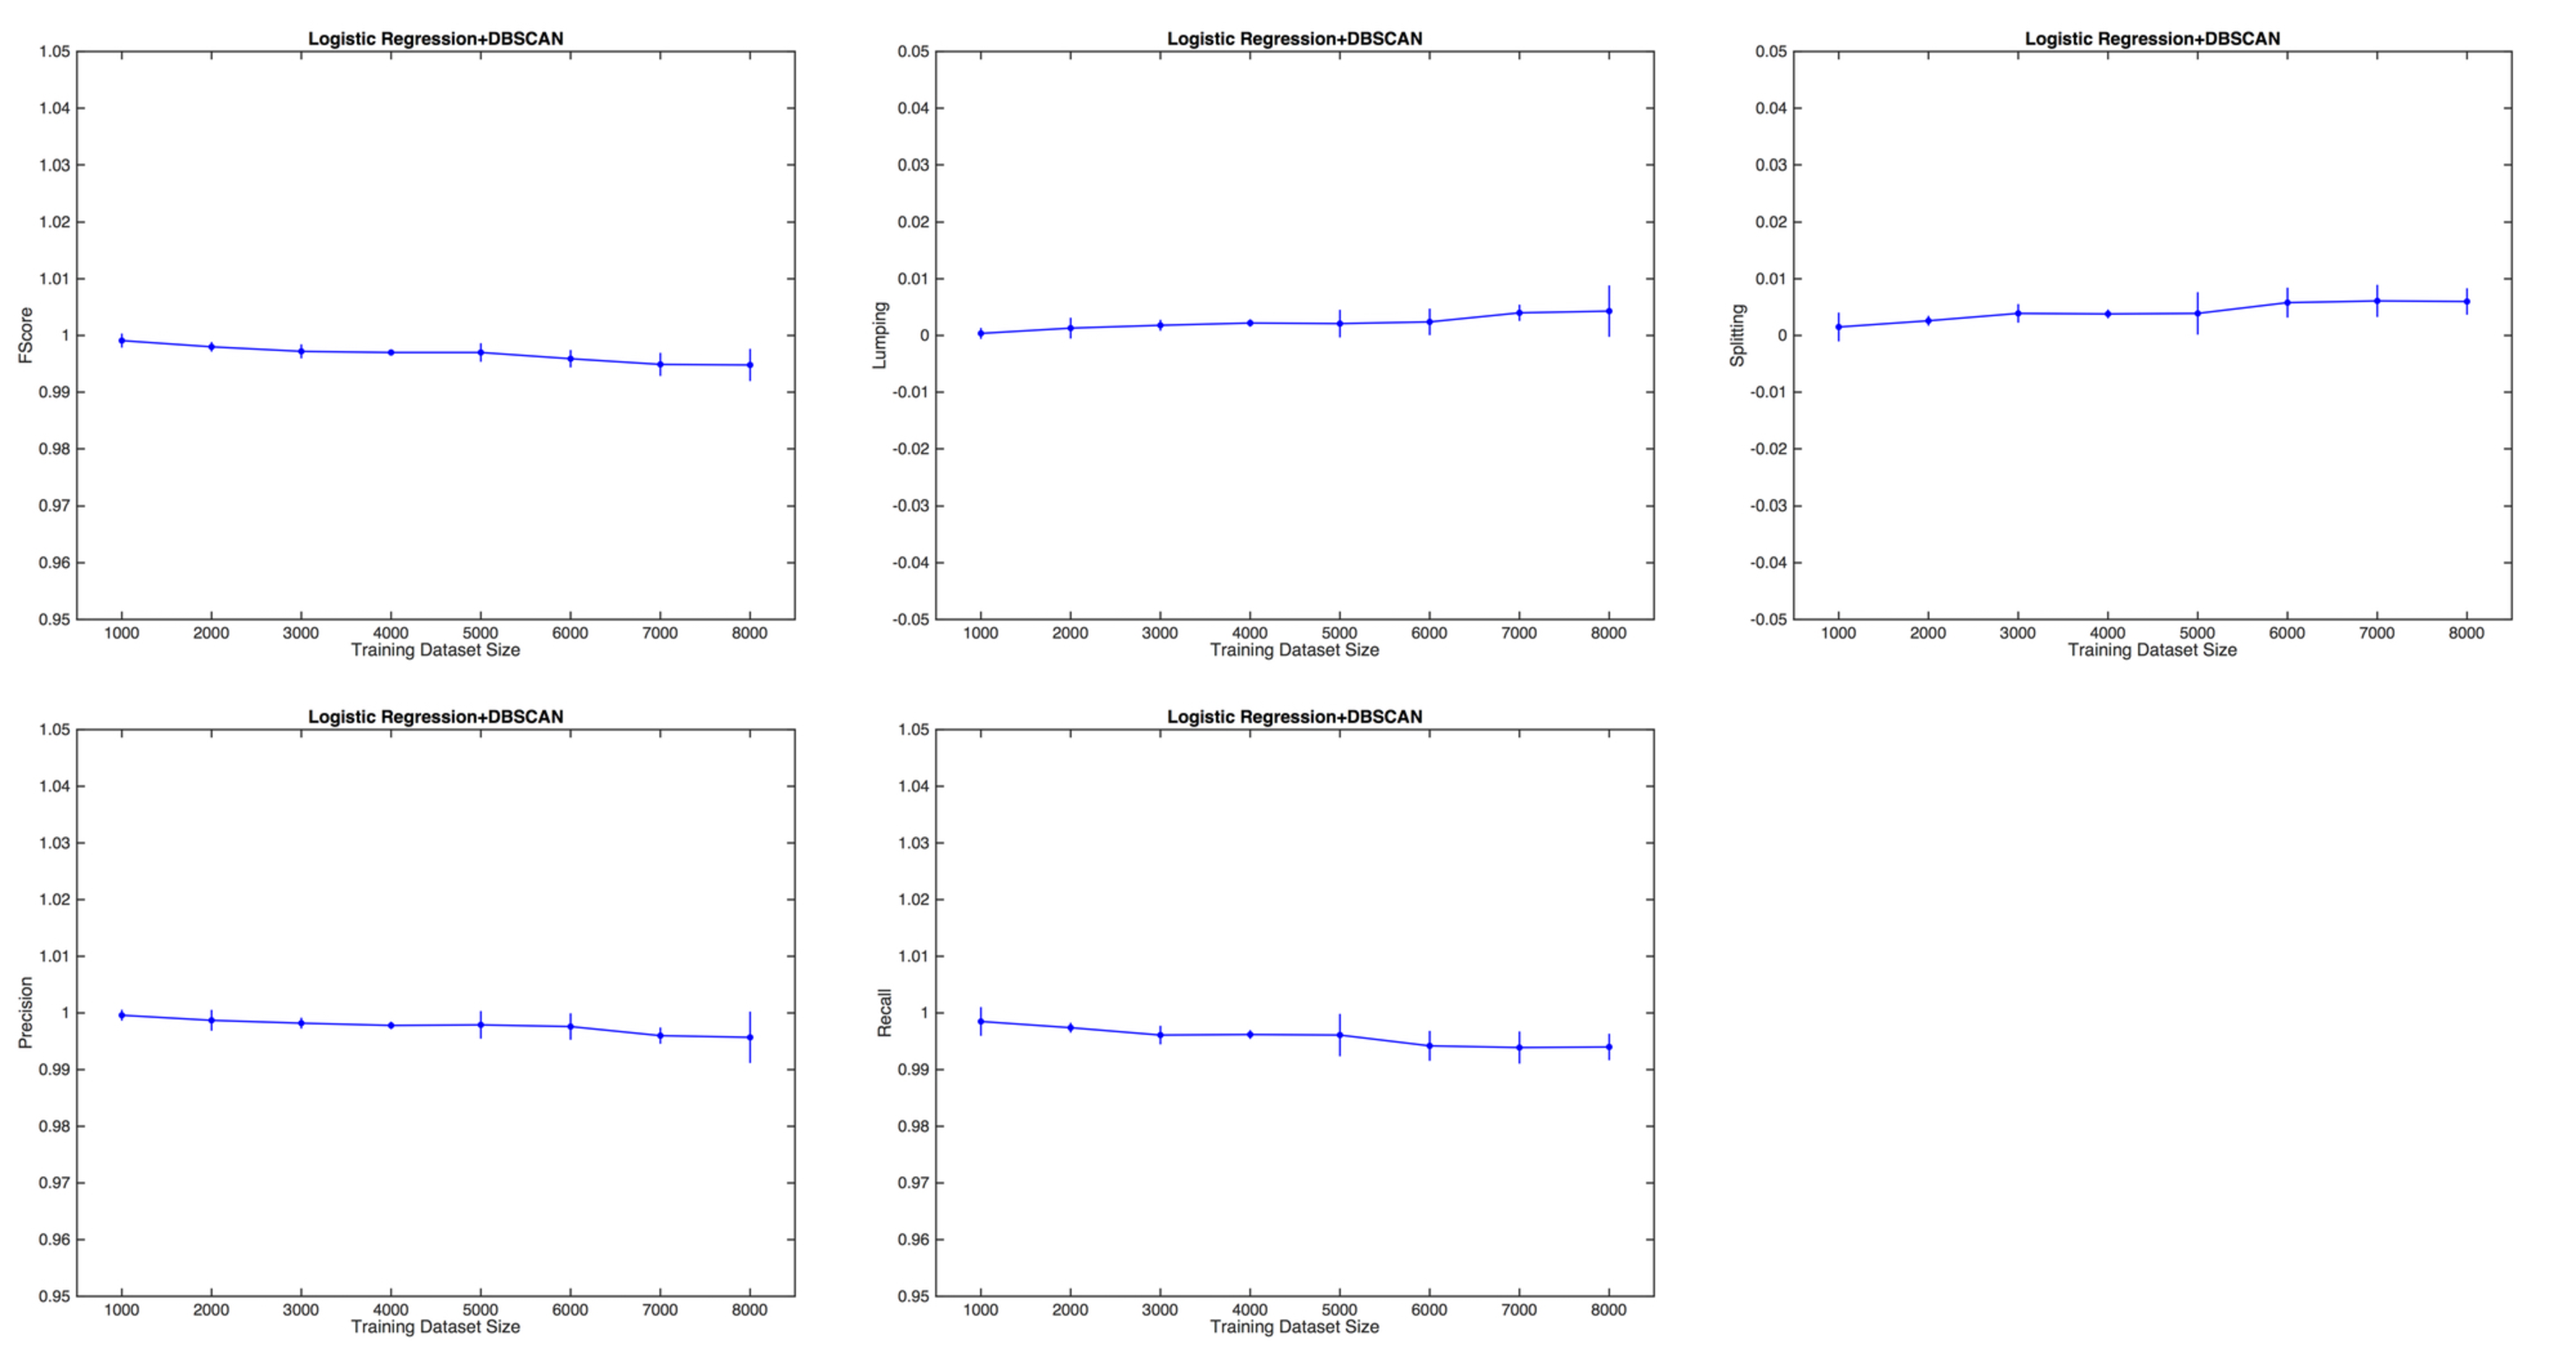
\includegraphics[scale=0.23]{CVDB.pdf}
\caption{Cross Validation for the Hierarchical Clustering}
\end{figure}
From the figure 5.1 and figure 5.2, the logistic regression with the clustering is stable. They also shows a good performance of the clustering result for the inventor identification. 

\begin{figure}
\centering
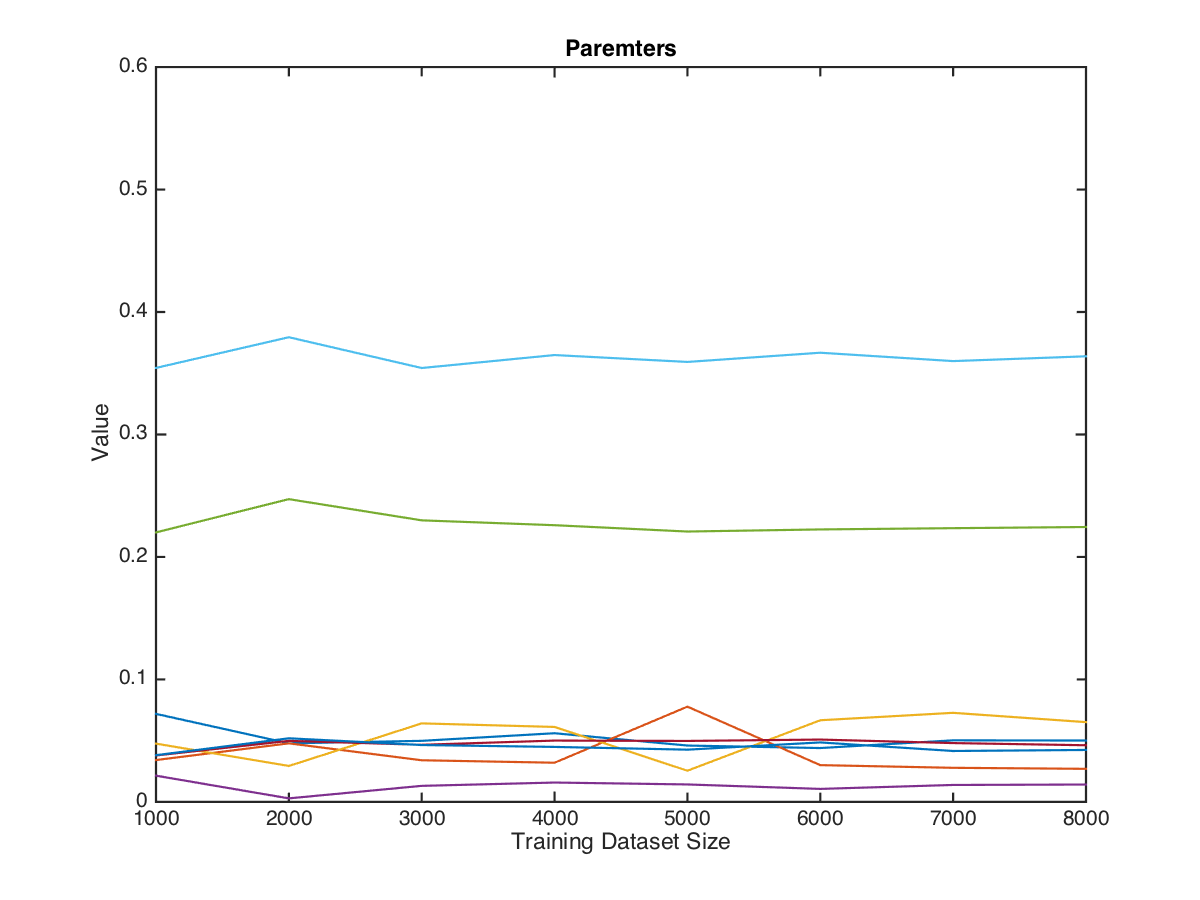
\includegraphics[scale=0.5]{parameters.png}
\caption{Parameters Values}
\end{figure}
 
The figure 5.3 shows the normalized parameters' values trained by the logistic regression with respect to different sizes of the training dataset. From the plot, the normalized parameters values  fluctuates when the size of the dataset changes. The changes is less than 0.1. The reason is that the subset is randomly chosen from the training dataset. Sometimes the subset of the training dataset is biased. When the size of the subset is larger than 6000, the fluctuation of the parameters decreases. From the experiment, the training dataset size should be larger than 6000 to get a stable result.

\subsection{Transitivity Effect}
The hierarchical clustering have three methods to calculate the cluster similarity and the DBSCAN can changes the minPts to affect the clustering result. They affect the clustering result by affecting the transitivity of inventor identity. In the second part, the transitivity effect is evaluated. The weights and threshold are the mean values of the cross validation of the whole training dataset from the first part of evaluation. A subset dataset which contains 5000 instances are randomly chosen from the testing dataset. For the hierarchical clustering, the three methods are evaluated by calculating the five measurements for them. The result is shown in the table 5.2. As it's explained before, the single-linkage clustering results in chain rule while the complete-linkage clustering avoids the chain rule. The transitivity of the average group linkage is between the single-linkage and the complete-linkage. From the table, the single-linkage has the best F-measurement and the complete-linkage has the worst F-measurement.  If the transitivity of the hierarchical clustering decreases, the F-measurement, the lumping error and the recall of the clustering result decrease, while the splitting error and the precision increase. If the transitivity increases, more instances are grouped into the same cluster. As a result, the splitting error decreases and the lumping error increases in the contrary. For the same reason, the precision increases and the recall decreases. Because the F-measurement is the main measurement, the single-linkage clustering shows the best performance compared to the other two method.

\begin{table}
\centering
\begin{tabular}{|c|c|c|c|c|c|}
\hline
&F1&Lumping&Splitting&Precision&Recall\\
\hline
Single Linkage& 0.99396&0.00336 &0.00870 &0.99662 &0.99130 \\
\hline
Average Group Linkage&0.99268 &0.00196 & 0.01259& 0.99802& 0.98740\\
\hline
Complete Linkage&0.98588 & 0.00112 & 0.02657 &0.99885 &0.97343 \\
\hline
\end{tabular}
\caption{Transitivity Effect of the Hierarchical Clustering}
\end{table}
\begin{figure}
\centering
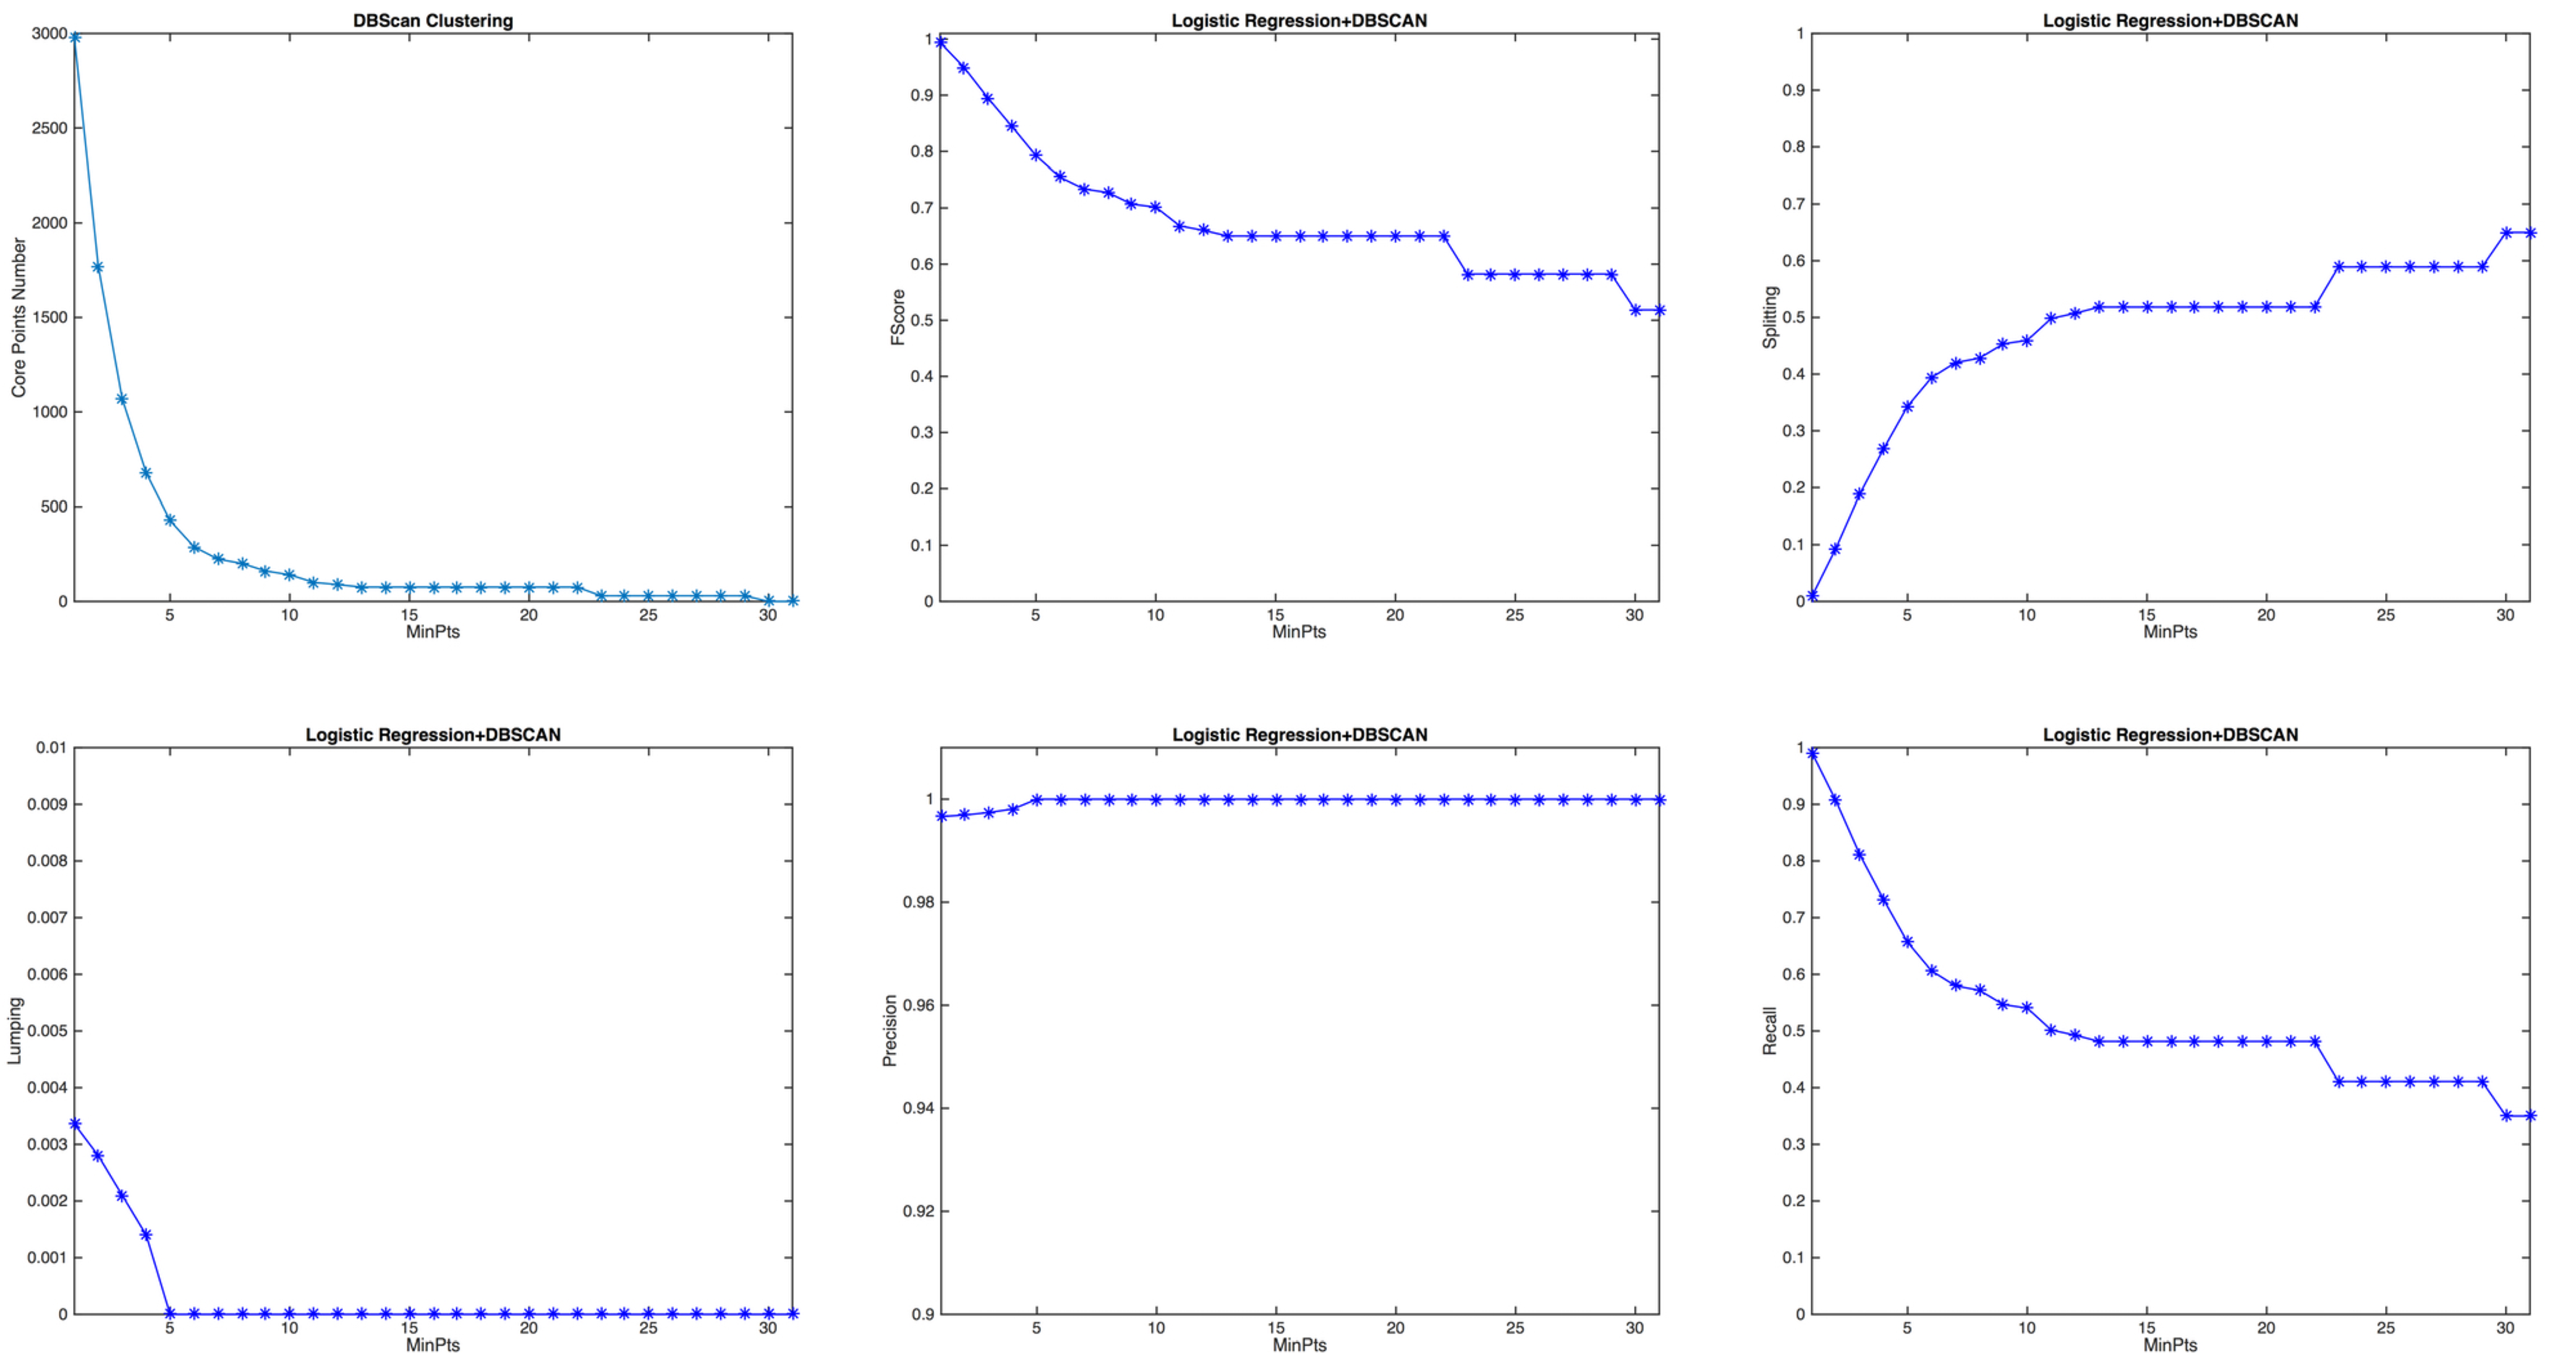
\includegraphics[scale=0.2]{DBSCANT.pdf}
\caption{DBSCAN Performance with respect to minPts}
\end{figure}

For DBSCAN, the radius is the threshold trained by the logistic regression. The minPts decides which inventor-patent instances are core objects for DBSCAN. The instances grouped into a cluster should be similar to at least one core object in the cluster. The minPts value affects the number of the core objects. The core objects affect the clustering result. From the figure 5.4, the core objects decreases as the value of minPts incrases. The precision increases and the lumping error decreases. After the minPts is larger than 5, the precision and the lumping error remains the same as 1 and 0. Which means. After the minPts reaches 5, the instances from the same clusters are all from the same inventors. The splitting error keeps increasing and the recall keeps decreasing as the minPts increases which means more and more instances from the same inventor are considered to be from different inventors.When the minPts reaches 30, the number of the core objects becomes 0. Each instance is put into a single cluster. The clustering result will not change any more. From the plot, the DBSCAN with the value 1 for minPts shows the best performance which has the best F-measurement. In conclusion, from the transitivity evaluation, the transitivity is proved to be helpful for improving the accuracy of the inventor identification.

\subsection{Clustering for Testing Dataset}
\begin{table}
\centering
\begin{tabular}{|c|c|c|c|c|}
\hline
F-Measurement&Lumping Error&Splitting Error&Precision&Recall\\
\hline
0.99151&0.01497&0.00212&0.98522&0.99788\\
\hline
\end{tabular}
\caption{Clustering Evaluation for the whole Testing Dataset}
\end{table}

From the second part of the evaluation, the single-linkage clustering and the DBSCAN with minPts 1 show the best performance. Therefore, they are chosen for the evaluation for the whole testing dataset. The values for the weights and threshold keep the same as the second part. For the third part, subsets are randomly chosen from the testing dataset with different sizes to test the clustering performance by calculating the five measurements. The size of the subset is from 2000 to 24495 and the increment is 2000. Figure 5.5 and Figure 5.6 show the performance of the DBSCAN and hierarchical clustering separately based on the five measurements. As it is explained before, setting minPts as 1 makes the DBSCAN clustering result same as the hierarchical clustering by using the single-linkage clustering method. The values of the F-measurement, precision and recall are around 0.99 with respect to the subset size of the testing dataset. The lumping error and splitting error is less than 0.02. The subset with the size 2000 has the worst F-measurement as 0.988 and the largest splitting error as 0.0159. This is because the subset is randomly chosen from the testing dataset. The small subset sometimes is biased. The table shows the five measurements for the whole testing dataset. Compared to the evaluation result of the USPTO PatentsView Inventor Disambiguation Workshop,the F-measurement,  precision and recall of the best performance on the E\&S dataset are 0.98279, 1 and 0.96616. However, the dataset of the evaluation for my approaches is the subset of the whole E\&S dataset. It's difficult to compare the evaluation result of my approach with theirs. It's still promising that my approach will have a good performance on the whole E\&S dataset.

\begin{figure}
\centering
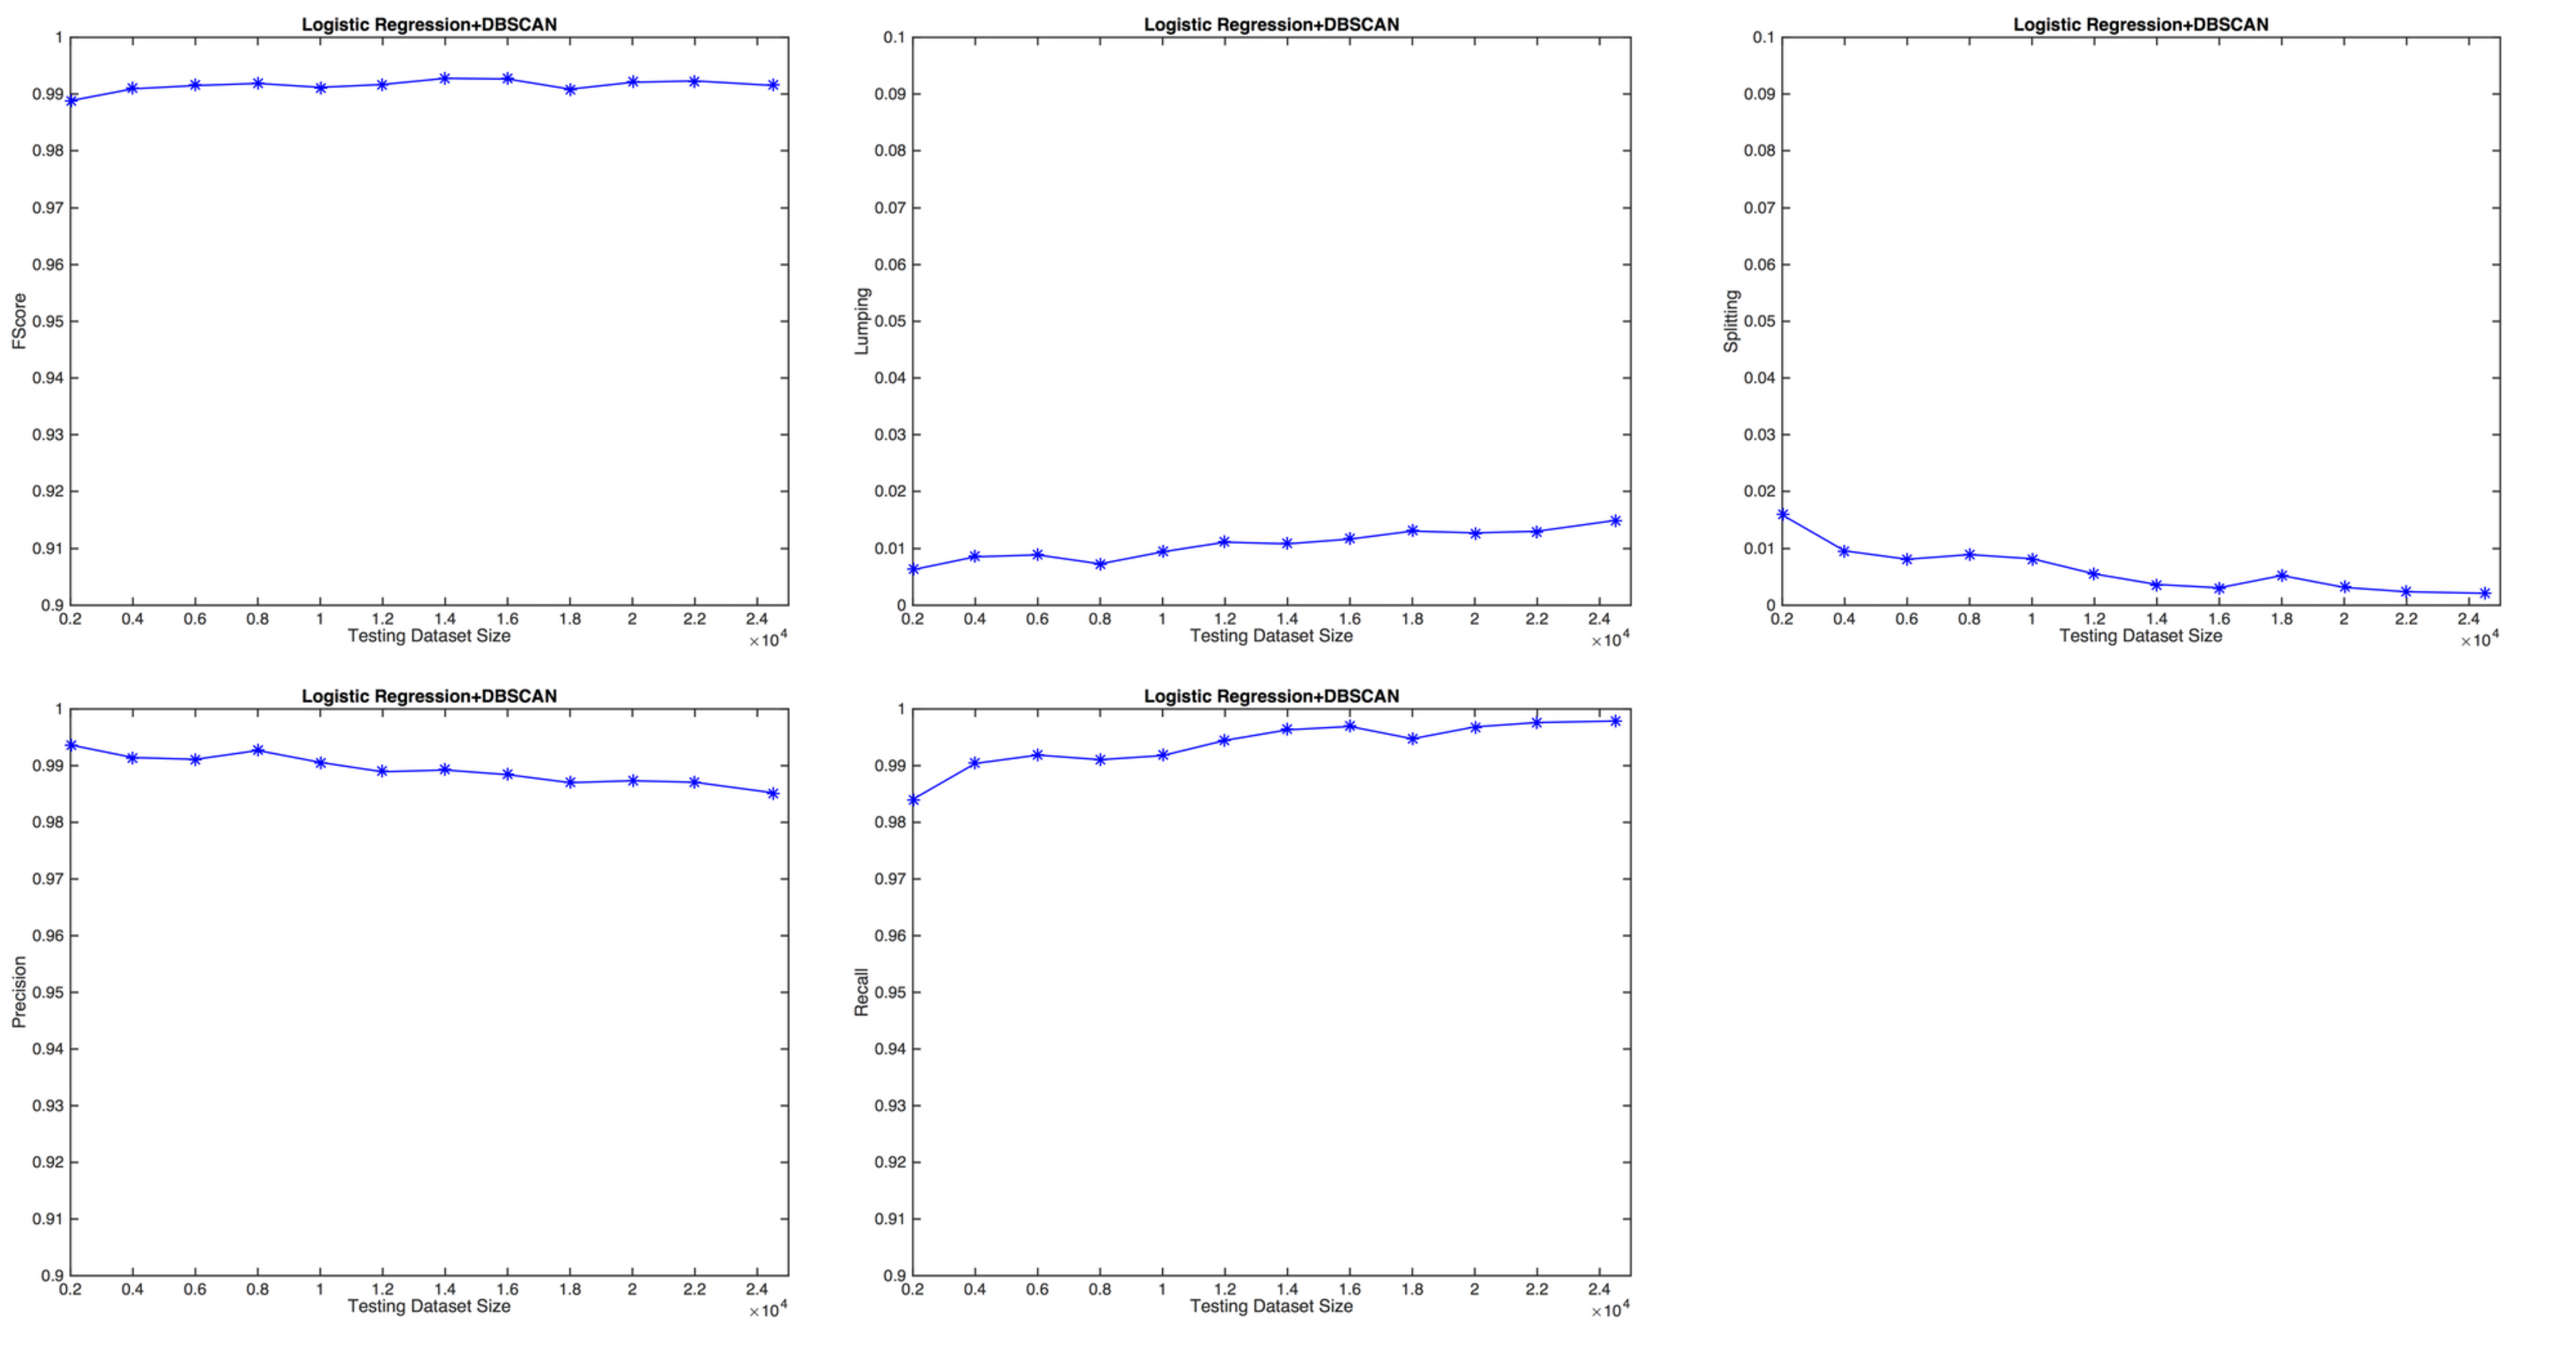
\includegraphics[scale=0.23]{DBTest.pdf}
\caption{DBSCAN Evaluation for Testing Dataset}
\end{figure}
\begin{figure}
\centering
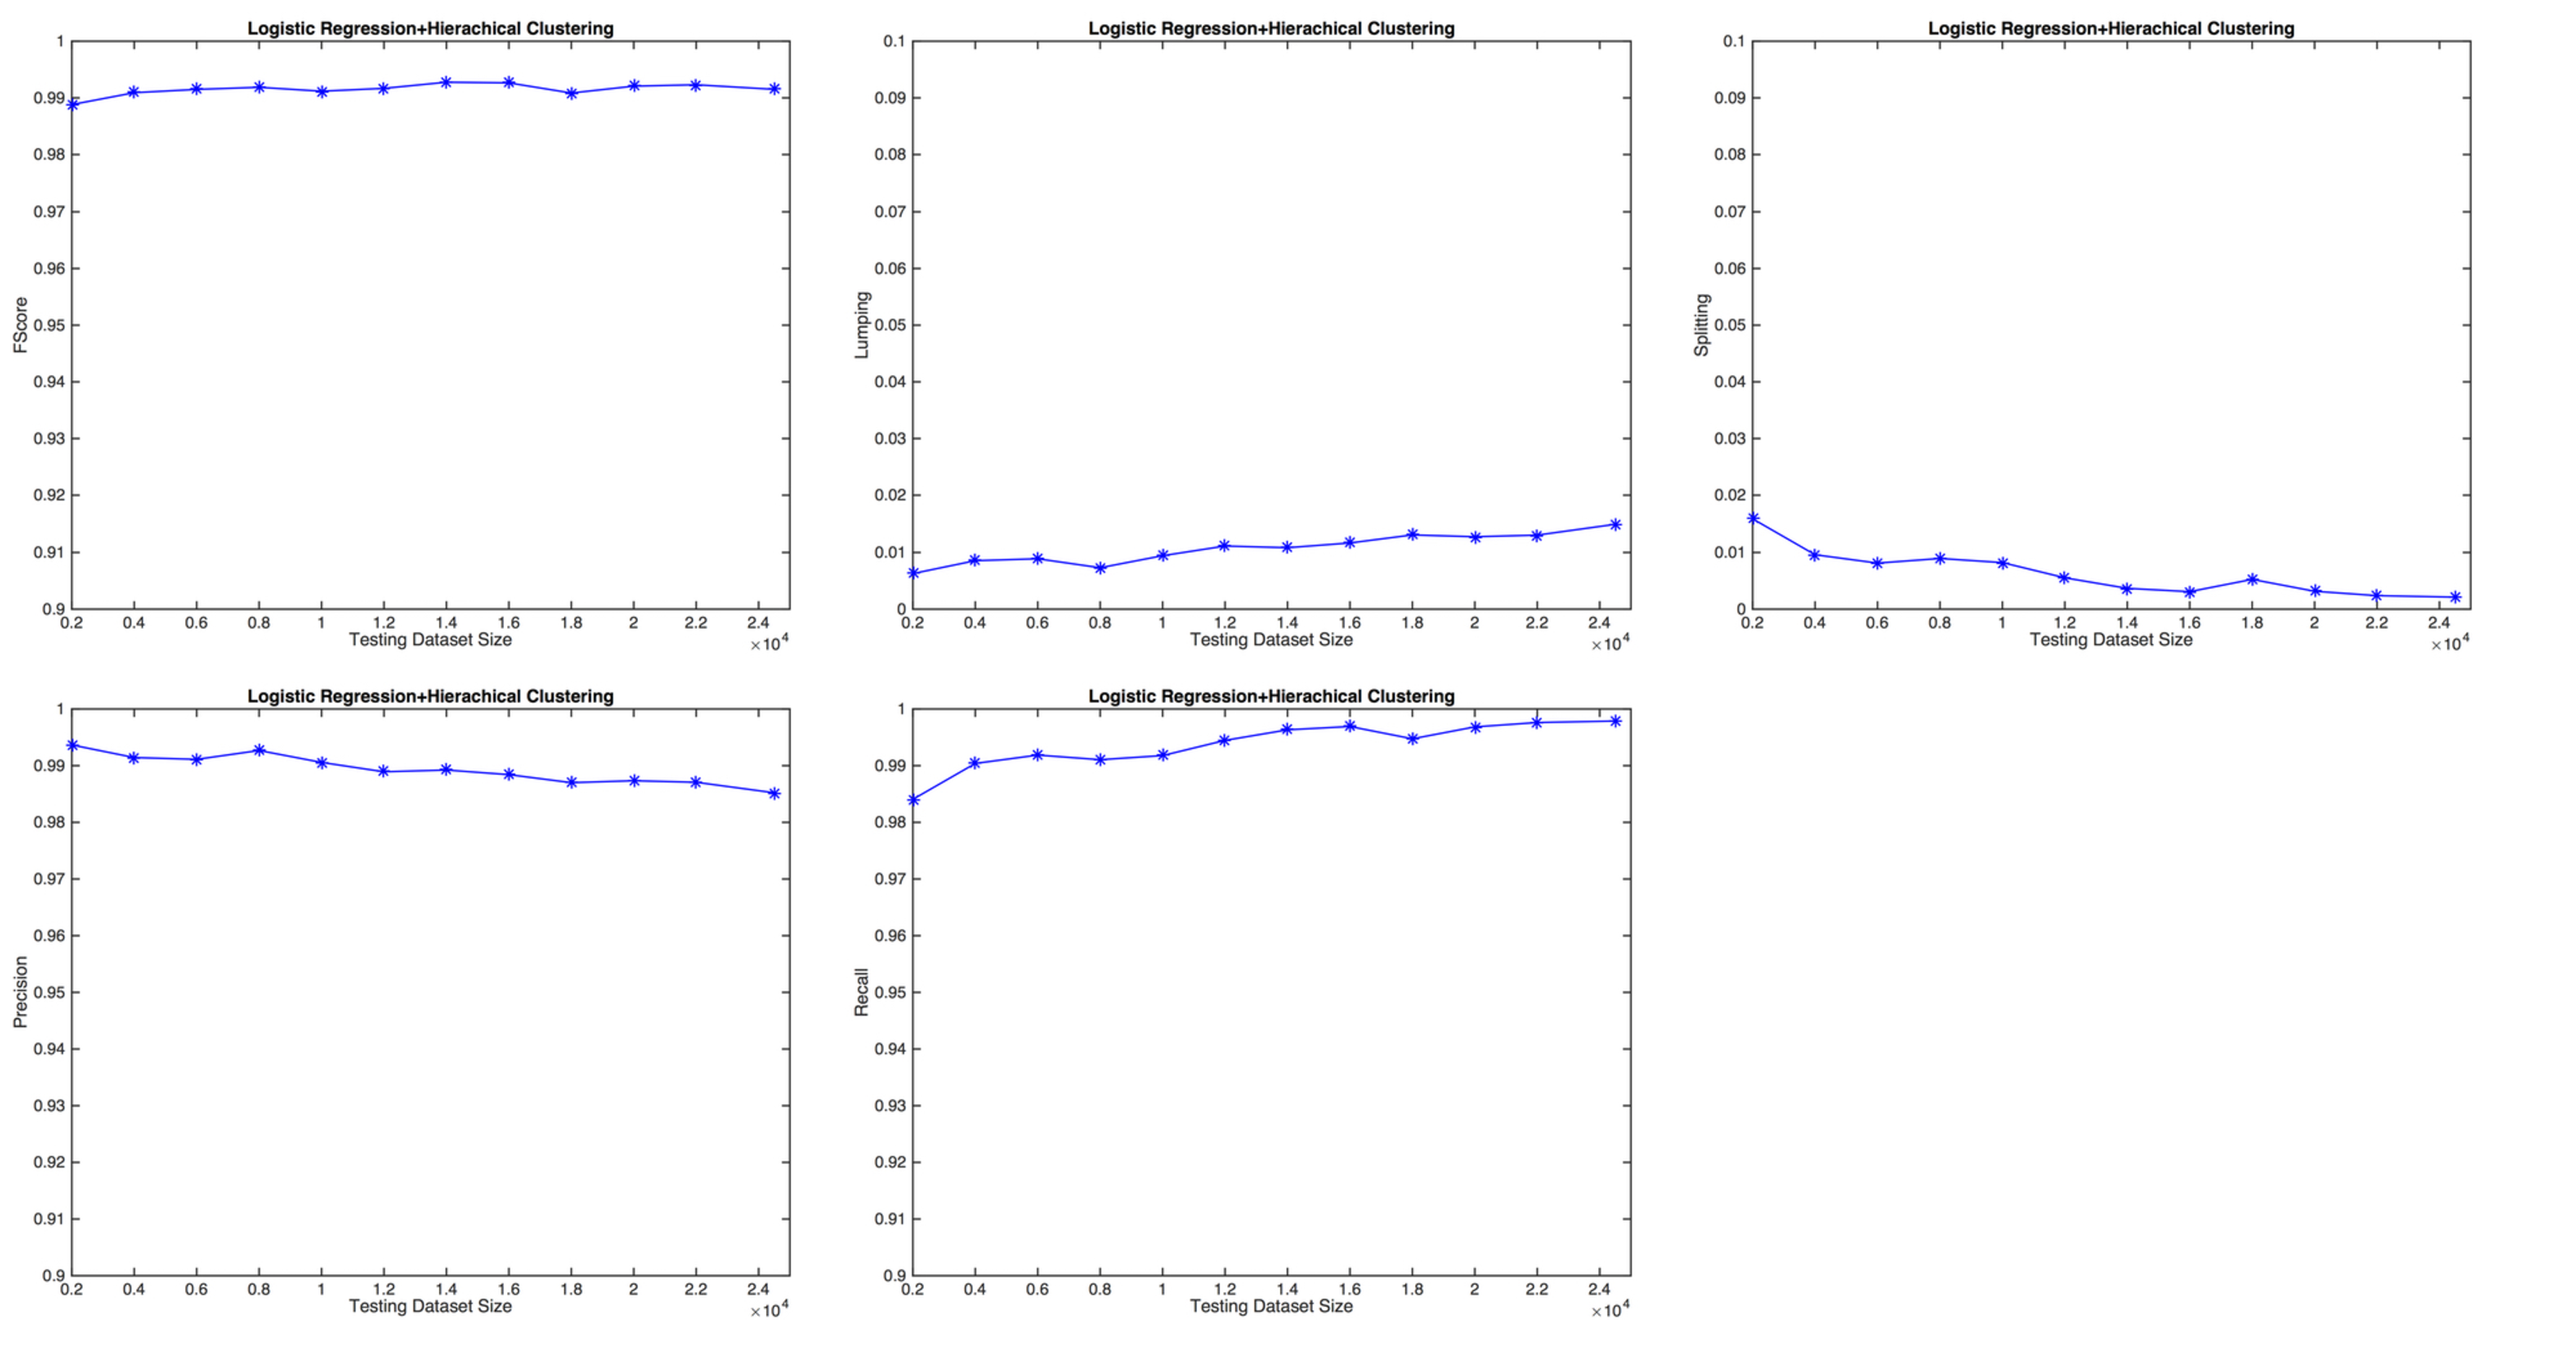
\includegraphics[scale=0.23]{HITest.pdf}
\caption{Hierachical Clustering Evaluation for Testing Dataset}
\end{figure}
   

\subsection{Comparison with the Flemming's approach}
Flemming uses a benchmark dataset to test the performance of his approach. The benchmark dataset contains 95 US inventors and 1332 inventor-patent instances.  Flemming's approach uses inventor name blocking techniques.  With different blocking rules, the approach give two different results for the inventor disambiguation which are named as \emph{Lower-bound} and \emph{Upper-bound}. In the fourth part of evaluation, my approach is used to do an inventor disambiguation for the benchmark dataset and compare my approach with the Flemming's. 
\begin{table}
\scriptsize
\begin{tabular}{|c|c|c|c|}
\hline
&F-Measuremen&Lumping Error&Splitting Error\\
\hline

\emph{Upper-Bound} (Flemming)&0.9744 &0.0150&0.0357\\

\hline

\emph{Lower-Bound}(Flemming)&0. 9764& 0.0150& 0.0319\\
\hline
Logistic Regression + (DBSCAN ,Hierarchical Clsutering) & 1.0 &0.0&0.0\\
\hline
\end{tabular}
\caption{Comparison with Flemming's Approach}
\end{table}
The table shows the F-measurement, lumping error and splitting error for the Flemming's \emph{upper bound} and \emph{lower bound} and my approach. All the inventors have been identified correctly by using my approach. The performance of my approach is better than the Flemming's on the benchmark dataset. 

\subsection{Publication-Patent Matching}
In the fifth part of the evaluation, the improvement for accuracy of clustering by using the publication patent matching is evaluated. The subset which contains 3604 instances from the intersection set of the Flemming's database and E\&S dataset is used. All these patents of the inventor-patent instances are from the bio-medical field in order to use the Europe PMC database.  The table 5.4 shows the evaluation result.
\begin{table} 
\scriptsize
\begin{tabular}{|c|c|c|c|c|c|}
\hline
&F-Measurement&Lumping Error&Splitting Error&Precision&Recall\\
\hline
Before patent-publication matching&0.9992&7.4056e-4&8.6398e-4&0.9993 &0.9991\\
\hline
After publication-patent matching&0.9992&7.4056e-4&8.6398e-4&0.9993 &0.9991 \\
\hline
\end{tabular}
\caption{patent-publication matching}
\end{table}

From the table, it shows that the patent-publication matching doesn't help to improve the accuracy of the clustering result. There are two reasons for that. First, the clustering result already shows almost correct inventor identification. An improvement for that is difficult. Second, the publication doesn't provide complete information for the author ID, abstract and affiliation and this increase the difficulty for the accuracy improvement. 